\documentclass[12pt]{beamer} %Makes presentation

%\documentclass[handout]{beamer} %Makes Handouts
\usetheme{Singapore} %Gray with fade at top
\useoutertheme[subsection=false]{miniframes} %Supppress subsection in header
\useinnertheme{rectangles} %Itemize/Enumerate boxes
\usecolortheme{seagull} %Color theme
\usecolortheme{rose} %Inner color theme

\definecolor{light-gray}{gray}{0.75}
\definecolor{dark-gray}{gray}{0.55}
\setbeamercolor{item}{fg=light-gray}
\setbeamercolor{enumerate item}{fg=dark-gray}

\setbeamertemplate{navigation symbols}{}
%\setbeamertemplate{mini frames}[default]
\setbeamercovered{dynamics}
\setbeamerfont*{title}{size=\Large,series=\bfseries}

%\setbeameroption{notes on second screen} %Dual-Screen Notes
%\setbeameroption{show only notes} %Notes Output

\setbeamertemplate{frametitle}{\vspace{.5em}\bfseries\insertframetitle}
\newcommand{\heading}[1]{\noindent \textbf{#1}\\ \vspace{1em}}

% small footnotes
\setbeamerfont{footnote}{size=\tiny}

\usepackage{bbding,color,multirow,times,ccaption,tabularx,graphicx,verbatim,booktabs,fixltx2e}
\usepackage{colortbl} %Table overlays
\usepackage[english]{babel}
\usepackage[latin1]{inputenc}
\usepackage[T1]{fontenc}
\usepackage{lmodern}
\usepackage{alltt}

\author[]{Thomas J. Leeper}
\institute[]{
  \inst{}%
  Department of Political Science and Government\\Aarhus University
}


\title{Reproducible Research with knitr}

\date[]{October 28, 2014}

\begin{document}

\frame{\titlepage}

\frame{\tableofcontents}

\section{Overview}
\frame{\tableofcontents[currentsection]}

\frame{
	\frametitle{Teaching/Learning Approach}
	\begin{itemize}\itemsep2em
		\item Hands-on practice
		\item Work independently to enhance your own workflow
		\item You will not learn everything today
	\end{itemize}
}

\frame{
	\frametitle{Outline for afternoon}
	\begin{itemize}\itemsep2em
		\item A short activity
		\item History and philosophy of literate programming
		\item Work through basics together
		\item Independent project work
		\item Wrap up and move forward
	\end{itemize}
}


\section{Activity}
\frame{\tableofcontents[currentsection]}

\frame{
	\frametitle{Think about your own workflow}
	\begin{itemize}\itemsep1.5em
		\item Think about: \textit{How do I get outputs from my data?}
		\item Draw a map or diagram of your workflow
		\item Include relevant steps and tools, such as:
			\begin{itemize}
				\item Tables
				\item Figures
				\item In-text citations and reference list
				\item In-text analysis summaries
				\item Cross-referencing (tables, figures, sections)
				\item Document layout
			\end{itemize}
		\item Make notes about areas that are \textit{time-consuming} and/or \textit{difficult}
	\end{itemize}
}



\section{Literate Programming}
\frame{\tableofcontents[currentsection]}

\frame{
	\frametitle{Literate programming}
	\begin{itemize}\itemsep1em
		\item Origins in computer program documentation
		\item Software source code should describe how to use that software
		\item Early tools
			\begin{itemize}
				\item \href{http://en.wikipedia.org/wiki/WEB}{WEB} by Donald Knuth (author of TeX)
				\item \href{http://en.wikipedia.org/wiki/Noweb}{noweb} by Norman Ramsey (1989)
			\end{itemize}
		\item Two operations to create two different outputs
			\begin{itemize}
				\item \textit{Weave}: Nice Documentation
				\item \textit{Tangle}: Executable code
			\end{itemize}
	\end{itemize}
}

\frame{
	\frametitle{Sweave}
	\begin{itemize}\itemsep2em
		\item Released in 2002 by Friedrich Leisch\footnote{\href{http://www.stat.uni-muenchen.de/~leisch/Sweave/Sweave-compstat2002.pdf}{Sweave: Dynamic Generation of Statistical Reports Using Literate Data Analysis}}
		\item Written for S (the language of R)
		\item Focused on creating articles
		\item Two operations to create two different outputs
			\begin{itemize}
				\item \texttt{SWeave}: LaTeX document (and PDF)
				\item \texttt{STangle}: Executable R code
			\end{itemize}
	\end{itemize}
}

\frame{
	\frametitle{knitr}
	\begin{itemize}\itemsep1em
		\item Released in 2012 by Yihui Xie\footnote{\href{http://yihui.name/knitr/}{knitr Homepage}}
		\item Conceptual descendant of Sweave
		\begin{itemize}
			\item Easier than Sweave
			\item Much more functionality and flexibility
		\end{itemize}
		\item Three operations to create two different outputs
		\begin{itemize}
			\item \texttt{knit}: PDF (and LaTeX document)
			\item \texttt{purl}: Executable R code
			\item \texttt{spin}: PDF (from pure R code)
		\end{itemize}
		\item Also create various outputs from non-LaTeX input
	\end{itemize}
}


\frame{
	\frametitle{How knitr Works\footnote{Image by \href{http://www.twitter.com/AriBFriedman}{Ari B. Friedman}}}
	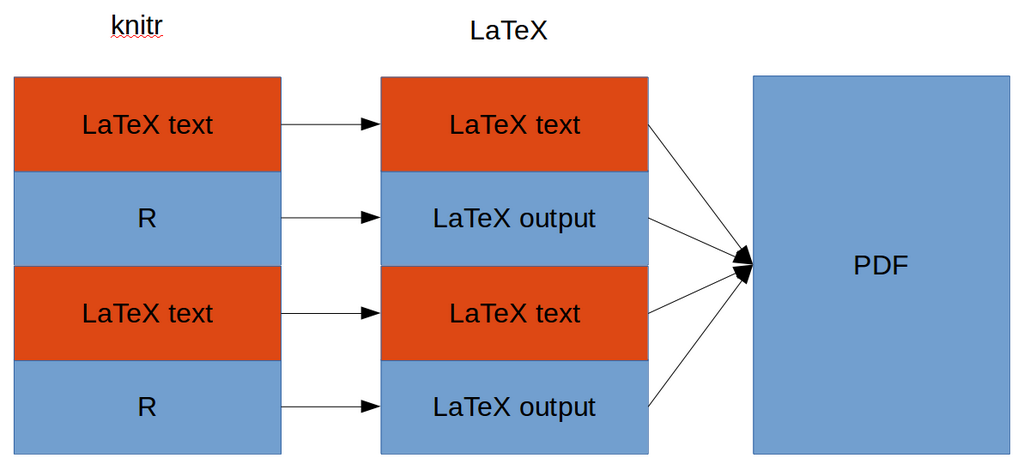
\includegraphics[width=\textwidth]{images/knitrprocess}
	% https://pbs.twimg.com/media/BvBO1s0IQAA5tDw.png:large
}


\frame{
	\frametitle{Workflows for knitr}
	\begin{center}
	\begin{tabular}{lcc}
		                & \textbf{Analysis} & \textbf{Output} \\ \midrule
		Irreproducible  &         R         &   Copy-paste    \\[1em]
		No knitr        &         R         & Manual includes \\[1em]
		Finish in knitr &         R         &  Load and knit  \\[1em]
		All knitr       &       knitr       &       n/a       \\[1em] \bottomrule
	\end{tabular}
	\end{center}
}

\frame{
	\frametitle{Workflows for knitr\footnote{Image by \href{http://www.twitter.com/AriBFriedman}{Ari B. Friedman}}}
	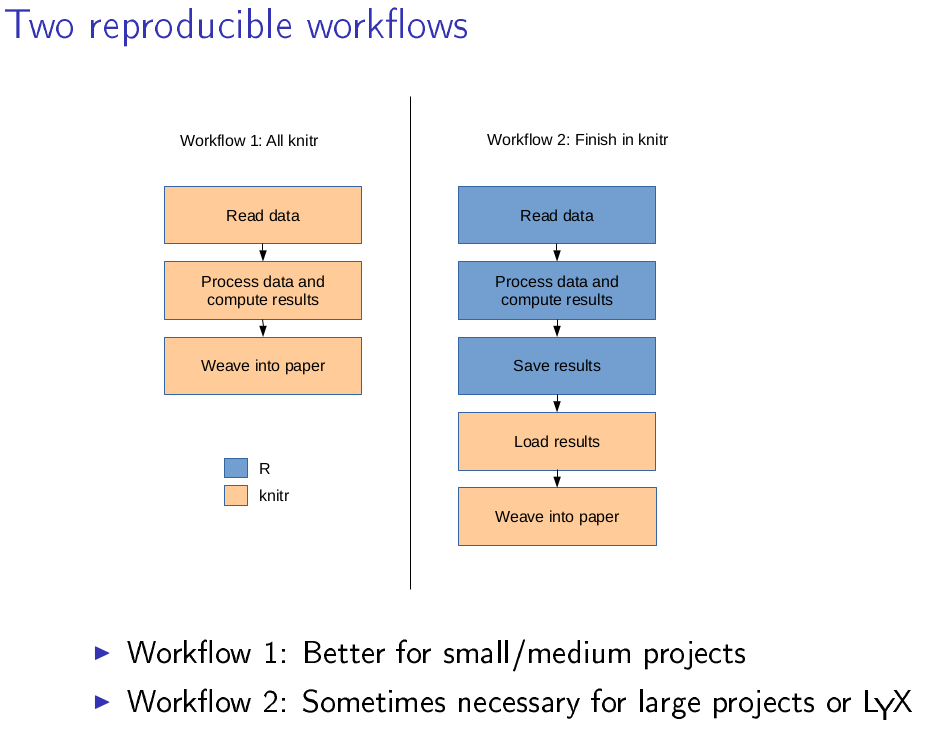
\includegraphics[width=\textwidth, trim = 0in 2in 0in 1.5in, clip]{images/knitrworkflow}
	% https://pbs.twimg.com/media/BvBUPapCUAIYMhW.png:large
}


\section{knitr in Depth}
\frame{\tableofcontents[currentsection]}

\frame{
	\frametitle{knitr Input}
	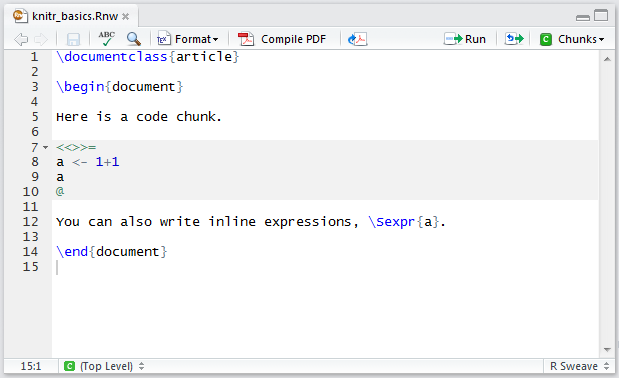
\includegraphics[width=\textwidth]{images/knitr-basic-knitr}	
}

\frame{
	\frametitle{PDF Output}
	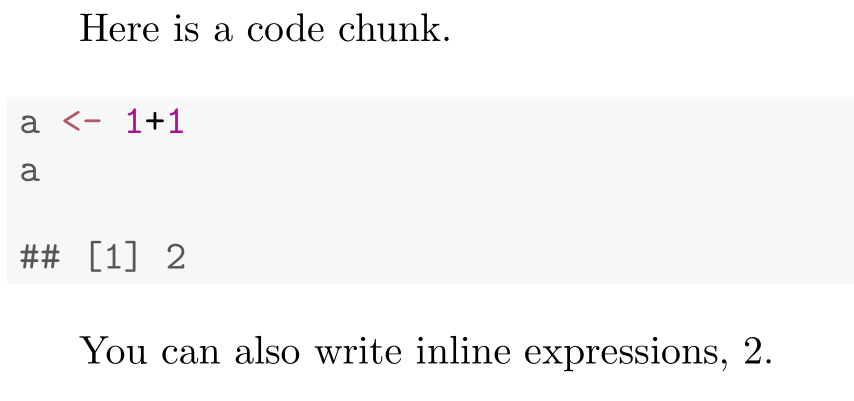
\includegraphics[width=\textwidth]{images/knitr-basic}
}

\frame{
	\frametitle{LaTeX Intermediary}
	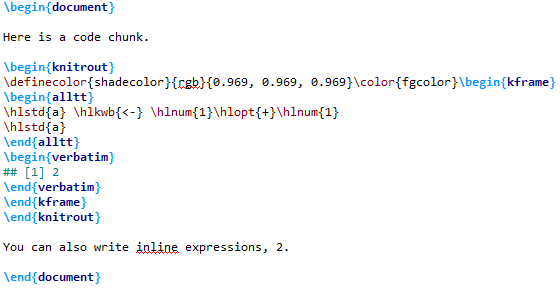
\includegraphics[width=\textwidth]{images/knitr-basic-latex}
}


\frame{
	\frametitle{Code Chunks}
	\begin{itemize}\itemsep2em
		\item Code chunks contain three parts
		\item Label
			\begin{itemize}
				\item Used for referencing chunks
			\end{itemize}
		\item Options
			\begin{itemize}
				\item Control chunk behavior and appearance
			\end{itemize}
		\item Contents
			\begin{itemize}
				\item R code to be evaluated
			\end{itemize}
	\end{itemize}
}

\frame{
	\frametitle{Code Chunks: Anatomy}
	{\large
	\begin{alltt}
	{\color<2>{red}<<}{\color<4>{red}a},{\color<5-6>{red}eval=TRUE},{\color<5,7>{red}echo=FALSE},{\color<5,8>{red}results='asis'}{\color<2>{red}>>=}
	
	{\color<3>{red} a <- 1+1\\a}
	
	{\color<2>{red}@}
	\end{alltt}
	}
}



\frame{
	\frametitle{Code Chunks: Options}
	\begin{itemize}\itemsep1.5em
		\item \texttt{echo}
		\item \texttt{eval}
		\item \texttt{results}
		\item \texttt{hold}
		\item \texttt{tidy} and \texttt{highlight}
		\item \texttt{warning} and \texttt{message}
	\end{itemize}
}

\frame{
	\frametitle{Code Chunks: Options}
	\begin{itemize}\itemsep2em
		\item Chunk options can be set for each chunk
		\item They can also be set globally in a document
    	\item E.g., \texttt{opts\_chunk\$set(echo = FALSE)}
	\end{itemize}
}

\frame{
	\frametitle{Code Chunks: Inline Code}
	\begin{itemize}\itemsep2em
		\item In addition to chunks, code can be written in-line
		\item Anything in \texttt{$\backslash$Sexpr\{\}} is evaluated
		\item Useful for in-line reporting of analyses
	\end{itemize}
}

\frame{
	\frametitle{Externalization}
	\begin{itemize}\itemsep2em
		\item Possible to \textit{externalize} R code
		\item ``Child'' documents
			\begin{itemize}
				\item Code chunks in separate file
			\end{itemize}
		\item Reading code chunks 
			\begin{itemize}
				\item Keep code in specially formatted R script
			\end{itemize}
	\end{itemize}
}


\frame{
	\frametitle{Chunk Caching}
	\begin{itemize}\itemsep2em
		\item knitr runs every chunk every time
		\item This is unnecessary if you're making non-code changes
		\item Can be time-consuming
		\item The \texttt{cache} chunk option changes this
	\end{itemize}
}

\frame{
	\frametitle{Chunk Caching: How it Works}
	\begin{itemize}\itemsep2em
		\item Set \texttt{cache=TRUE} to \textit{cache} a chunk
		\item knitr stores the chunk and its results
    		\begin{itemize}
        		\item Stored in .RData files in \texttt{./cache}
    		\end{itemize}
		\item Cached chunks are only run after changes
    		\begin{itemize}
        		\item Substantive and non-substantive changes
    		\end{itemize}
		\item Behavior depends on relations between chunks
	\end{itemize}
}

\frame{
	\frametitle{Chunk Caching: Chunk Dependencies}
	\begin{itemize}\itemsep2em
		\item Cached chunks are only rerun if modified
		\item But chunks might depend on other chunks
    		\begin{itemize}
        		\item B depends on cached A
        		\item Cached B depends on A
        		\item Cached B depends on cached A
    		\end{itemize}
    	\item Specify dependencies with \texttt{dependson}
        	\begin{itemize}
            	\item Or: \texttt{opts\_chunk\$set(cache=TRUE, autodep=TRUE)}
        	\end{itemize}
	\end{itemize}
}


\frame{
	\frametitle{Figures}
	\begin{itemize}\itemsep1em
		\item Two ways to include figures:
		\item Using knitr chunk options for figures
			\begin{itemize}
				\item Handles lots of details automatically
				\item Takes work to customize
			\end{itemize}
		\item Manually using \texttt{$\backslash$includegraphics\{\}}
			\begin{itemize}
				\item Somewhat finer control
				\item Requires more LaTeX overhead
			\end{itemize}
	\end{itemize}
}


\frame{
	\frametitle{Tables}
	\begin{itemize}\itemsep2em
		\item LaTeX tables are tedious
		\item Doing them by-hand is irreproducible and a waste of time
		\item Lots of ways to create tables with knitr
		\begin{itemize}
			\item \texttt{kable}
			\item \texttt{xtable}
			\item \texttt{stargazer}
		\end{itemize}
	\end{itemize}
}


\frame{
	\frametitle{Porting a Project to knitr}
	\begin{itemize}\itemsep2em
		\item Move existing R code into a knitr framework
		\item What code chunks and in-line expressions do you need
		\item How do you create tables and figures?
	\end{itemize}
}


\frame{
	\frametitle{Package Versioning}
	\begin{itemize}\itemsep2em
		\item Reproducibility requires knowing software used to conduct analyses
		\item Including package names using \texttt{library} or \texttt{require} is not enough
		\item Your future self (and others) need to know package versions
		\item How do we handle that?
	\end{itemize}
}

\frame{
	\frametitle{Package Versioning: Do it Manually}
	\begin{itemize}\itemsep2em
		\item Record versions and either:
			\begin{itemize}
				\item Put these in a README
				\item Have knitr fail on wrong version
			\end{itemize}
		\item Manually install package version:
			\begin{itemize}
				\item \href{http://cran.r-project.org/web/packages/devtools/index.html}{devtools}
				\item \href{http://cran.r-project.org/web/packages/repmis/index.html}{repmis}
			\end{itemize}
		\vspace{1em}
		\item Tedious
	\end{itemize}
}

\frame{
	\frametitle{Package Versioning: packrat}
	\begin{itemize}\itemsep2em
		\item Package developed by RStudio
		\item Work in an isolated software environment
		\item Install packages into a local project directory
		\vspace{1em}
		\item Share your \textbf{packrat} directory as part of your reproducible directory
	\end{itemize}
}

\frame{
	\frametitle{Package Versioning: checkpoint}
	\begin{itemize}\itemsep2em
		\item Package developed by Revolution Analytics
		\item Register a ``checkpoint'' (a date) for your analyses
		\item All packages are drawn from MRAN, a daily snapshot of the R package universe
		\vspace{1em}
		\item No need to store/share a large package directory
	\end{itemize}
}

\section{Wrapup}
\frame{\tableofcontents[currentsection]}


\frame{
	\frametitle{Wrapup}
	\begin{itemize}\itemsep2em
		\item What questions/concerns do you have?
		\item How have today's activities helped you think about your own reproducible workflow?
	\end{itemize}
}

\appendix
\frame{}


\section{Go Next}
\frame{
	\frametitle{Things we probably didn't cover}
	\begin{itemize}\itemsep1.5em
		\item knitr's \texttt{spin} function: Creates a PDF from an R script
			\begin{itemize}
				\item Really useful for teaching assignments
			\end{itemize}
		\item Language engines: Embed non-R code
			\begin{itemize}
				\item Python, Bash, Julia, FORTRAN, Stata(?)
			\end{itemize}
		\item rmarkdown: knit without using LaTeX markup
	\end{itemize}
}

\section{Other Tools}
\frame{
	\frametitle{Other Reproducible Research Tools}
	\begin{itemize}\itemsep1em
		\item \href{http://git-scm.com/}{git}: Version control
		\item \href{https://github.com/}{GitHub} and \href{https://bitbucket.org/}{Bitbucket}: Git cloud services
    		\begin{itemize}
    		\item Good for collaboration\footnote{\href{http://thomasleeper.com/2014/07/git-bitbucket-word-collaboration/}{See ``Collaborating with Git and Bitbucket''}}
    		\end{itemize}
		\item \href{http://johnmacfarlane.net/pandoc/}{pandoc}: Command-line tool to convert documents between formats
		\item Tools for R package versioning
			\begin{itemize}
				\item \href{http://cran.r-project.org/web/packages/devtools/index.html}{devtools}
				\item \href{http://cran.r-project.org/web/packages/repmis/index.html}{repmis}
				\item \href{http://cran.r-project.org/web/packages/packrat/index.html}{packrat}
				\item \href{http://cran.r-project.org/web/packages/checkpoint/index.html}{checkpoint}
			\end{itemize}
	\end{itemize}
}

\section{knitr Resources}
\frame{
	\frametitle{knitr Resources}
	\begin{itemize}\itemsep1.5em
		\item \href{http://yihui.name/knitr/}{knitr website}
		\item \href{http://cran.r-project.org/web/views/ReproducibleResearch.html}{CRAN Reproducible Research TaskView}
		\item \href{http://www.amazon.com/gp/product/1482203537}{\textit{Dynamic Documents with R and knitr}}
		\item \href{http://www.amazon.com/Reproducible-Research-RStudio-Chapman-Series/dp/1466572841/ref=pd\_bxgy\_b\_text\_y}{\textit{Reproducible Research with R and RStudio}}
		\item \href{https://groups.google.com/forum/\#!forum/knitr}{knitr Google} Group
		\item \href{http://stackoverflow.com/questions/tagged/knitr}{knitr on StackOverflow}
	\end{itemize}
}



\appendix
\frame{}

\end{document}
